
\begin{figure}
    \centering
    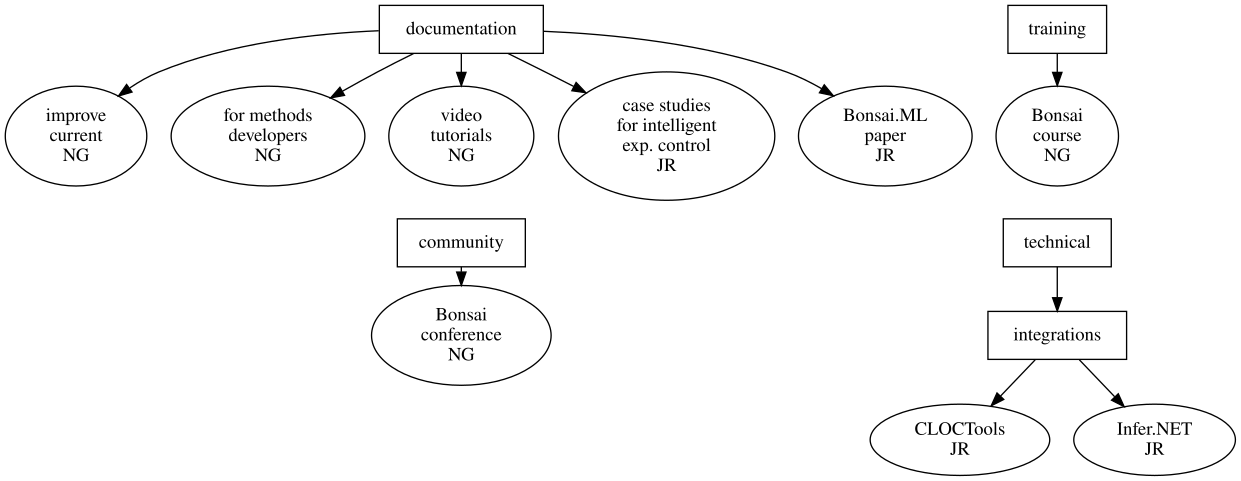
\includegraphics[width=6in]{activitiesGraphs/activities_larger.png}

    \caption{Proposed activities. The initials below each task name indicate
    the responsible team member (JR: Joaquin Rapela, NG: NeuroGEARS Ltd). See
    text for details.}

\end{figure}

\subsection{Approach}

\subsubsection{Aim 1: Documentation}

\paragraph{Summary:} Refactor the existing Bonsai.ML documentation and add new examples, user guides, troubleshooting resources, and video tutorials.

\paragraph{Background:} The Bonsai.ML project has maintained a strong commitment to producing high-quality documentation. However, the interdisciplinary nature of the project, supporting both experimental neuroscience users and machine learning method developers, has led to challenges in structuring the documentation for effective use. Currently, the documentation includes installation guides for each package, an automatically generated API reference for the C\# codebase, and a few examples demonstrating various use cases. Crucially, the documentation lacks good statistical descriptions of the implemented models developed so far, with no clear resources explaining core machine learning concepts and no resources for guiding users on how to implement machine learning pipelines for their specific applications. This has led to confusion among users who are struggling to find the information they need to effectively get started using Bonsai.ML.

Our team has been approached by several users of the package expressing concerns about the current state of the documentation, particularly regarding its structure. There is redundancy in certain places across various pages of the documentation and a lack of clarity in others. For instance, the installation instructions for various packages is included in both the "Getting Started" section of the examples and in the installation articles. Furthermore, the documentation site lacks critical statistical information that is essential for understanding the functionality of the package and use-cases. This lack of clarity and redundancy has made it difficult for users to find the information they need, leading to unnecessary user friction and driving people away from using our packages.

The confusion around documentation is exacerbated by the fact that machine learning method developers looking to introduce new functionality into Bonsai cannot find guidance on how to integrate their own machine learning models. While our team has discovered several approaches for best practices to integrate machine learning models into Bonsai, this information is currently siloed or distributed across various sources, including GitHub repos, discussion issues, pull requests, and undocumented communications. The Bonsai.ML project would greatly benefit from a dedicated, centralized resource that can provide documentation for method developers looking to introduce new machine learning functionality into Bonsai using the approaches our team has developed.

\paragraph{Previous work:} The current Bonsai.ML documentation was developed by the project team using the existing Bonsai documentation as a template. While this provided a solid foundation for getting started, the unique requirements of the Bonsai.ML project necessitate a more comprehensive, tailored form of documentation. To inform our restructuring efforts, we have reviewed the documentation of leading machine learning libraries, including \href{https://scikit-learn.org/stable/documentation.html}{scikit-learn}, \href{https://pytorch.org/docs/stable/index.html}{PyTorch}, and \href{https://tensorflow.org/learn}{TensorFlow}. We will draw inspiration from these examples to restructure and enhance the Bonsai.ML documentation, ensuring it meets the needs of both experimental neuroscientists and machine learning developers.

\paragraph{Tasks:}\mbox{}\\

\begin{description}

    \item[doc\_review:] Conduct a thorough review of the existing Bonsai.ML documentation. Identify redundancies, outdated content, and missing sections compared to other machine learning libraries, such as \href{https://scikit-learn.org/stable/documentation.html}{scikit-learn}, \href{https://pytorch.org/docs/stable/index.html}{PyTorch}, \href{https://tensorflow.org/learn}{TensorFlow}, and \href{https://docs.microsoft.com/en-us/dotnet/machine-learning/}{ML.NET}.

    \item[doc\_style\_guide:] Create a Bonsai.ML style guide which will include conventions for: documentation, code formatting, naming, and video tutorial formatting. These will draw on inspirations from the style guides and best practices put forth by \href{https://learn.microsoft.com/en-us/dotnet/csharp/fundamentals/coding-style/coding-conventions}{Microsoft}, the \href{https://github.com/dotnet/runtime/blob/main/docs/coding-guidelines/coding-style.md}{dotnet community}, and the developers of \href{https://github.com/pytorch/pytorch/blob/main/CONTRIBUTING.md}{PyTorch}.
    
    \item[doc\_examples\_improvement:] Improve the existing examples by restructuring them to match the new style guide. Each example will include a detailed explanation of the Bonsai workflow, the mathematical/statistical basis of the model, and clarifications on assumptions and data requirements.

    \item[doc\_examples\_new:] Develop at least 3 new examples that showcase complete applications of Bonsai.ML. These examples will cover: neural signal processing, real-time latent visualization, and clustering of behavioural data. Each example will have detailed workflow descriptions, information on the models and assumptions, and explanations of the datasets.

    \item[doc\_user\_guides:] Write new, comprehensive user guides to teach users about key ML concepts and how to use the Bonsai.ML libraries correctly. User guides will come in 2 flavours: one will be geared towards neuroscientists who may have familiarity with conducting experiments but are less familiar with ML techniques. These will focus more on teaching core concepts of math, statistics, and machine learning. The other style will be geared more towards ML developers and will focus more on reactive, online data streams and approaches for integrating ML models into Bonsai. These user guides will include how to create a new Bonsai.ML package with Python, C\# and expression scripting, and integrating models via TorchSharp and other native C\# libraries.
    
    \item[doc\_troubleshooting:] Create a troubleshooting section to address common issues users may encounter when using Bonsai.ML packages. This section will include solutions to frequently asked questions, common errors, and tips for debugging.
    
    \item[doc\_videos:] Produce at least 3 video tutorials and demos, hosted on YouTube, and embed them directly into the documentation. These videos will cover key topics such as installation, user guides, and examples. The 3 videos will be: 1) Installation and getting started with Bonsai.ML, 2) Integrating custom models into Bonsai using Python, C\#, and TorchSharp, and 3) Building a Bonsai.ML application to perform closed-loop stimulation using online neural signal processing.

\end{description}

\paragraph{Impact:}
Improving the documentation of Bonsai.ML will directly improve the code's maintainability, reduce technical debt for maintainers and contributors, and expand the project's reach. The expansion of the documentation will also greatly enhance usability of Bonsai.ML for two core communities: experimental neuroscientists and machine learning developers. Clearer, better-structured resources aimed at these groups will reduce barriers to usage and onboarding friction. We will provide user guides for experimental neuroscientists to learn the concepts underlying machine learning methods so they may use these methods for real-time experimental applications. Additionally, we will provide machine learning method developers with resources to guide them towards integrating new functionality into Bonsai. By adding examples, comprehensive user guides, troubleshooting resources, and video tutorials, we will create robust, easy-to-navigate documentation, modeled after leading ML libraries, that will greatly improve Bonsai.ML's sustainability and adoption.

\paragraph{Milestones and Indicators:}\mbox{}\\

\begin{description}

    \item[doc\_m1]: Documentation review completed and style guide released.
    \item[doc\_i1]: Publically shared document on GitHub detailing review of current documentation and plan for restructuring. Style guide publicly shared at docs/contributing.md on GitHub which will include information on coding style, contributing code/PRs, documentation, unit testing, and naming conventions.
    
    \item[doc\_m2]: All existing examples reviewed and updated to conform to the style guide.
    \item[doc\_i2]: All existing examples updated with new documentation to address missing information on mathematical/statistical background, data assumptions, and Bonsai workflows.
    
    \item[doc\_m3]: Three new examples published (neural signal processing, real-time latent visualization, behavioural clustering).
    \item[doc\_i3]: Each new example will be documented with explanation of the workflow components, mathematical basis of models/algorithms, and assumptions about the data.
    
    \item[doc\_m4]: New user guides and troubleshooting sections published.
    \item[doc\_i4]: At least 3 user guides developed per audience type completed (3 user guides tailored towards neuroscientists and explaining core ML concepts, 3 user guides for ML developers explaining how to integrate models into Bonsai). Troubleshooting section will include at least 10 common issues/errors addressed.
    
    \item[doc\_m5]: Video tutorials produced, uploaded to YouTube, and embedded in documentation.
    \item[doc\_i5]: Video 1: "Installation and Getting Started with Bonsai.ML" - posted by April. Video 2: "Integrating Custom Models with Python, C\#, and TorchSharp" - posted by May. Video 3: "Building a Closed-Loop Experiment with Bonsai.ML." - posted by September. Video engagement will be monitored by tracking views, likes, and comments.

\end{description}

\noindent\rule{\textwidth}{1pt}
\subsubsection{Aim2: Training}
\paragraph{Summary:} Organise a Bonsai course with a dedicated Bonsai.ML module.

\paragraph{Previous work:} Since 2017, NeuroGEARS Ltd has organised at least
two Bonsai courses per year at different universities, and deliver a
one-week-long Bonsai course, hosted at the Sainsbury Wellcome Centre, for
approximately 20 students, targeted to Bonsai users with intermediate
understanding of the language. The structure of the course will be similar to
previous ones (e.g., \href{https://neurogears.org/st-andrews-2024/}{2024 Bonsai
Course at St.~Andrews University}) and is outlined briefly below.

\begin{description}
    \item[Day 1 - Introduction to Bonsai:] What is visual reactive programming? Introduction to Marble diagrams and how to read them. Learning your way around the Bonsai IDE. How to measure and control almost anything with Bonsai. Real-time tracking of colored objects, moving objects and contrasting objects. Measuring behavior using voltages and an Arduino.

    \item[Day 2 - Real-time closed-loop experiments:] Fundamental reactive operators. Data synchronization and measuring closed-loop latency. Conditional effects: triggering a stimulus based on video activity. Continuous feedback: modulate stimulus intensity with speed or distance. Continuous and conditional feedback: closed-loop experiment building blocks. Synchronising asynchronous data streams.

    \item[Day 3 - Operant behavioral tasks:] Sharing observable sequences. Creating dynamic observable sequences with higher-order operators. Modeling trial sequences: states, events, and side-effects. Driving state transitions with external inputs. Best practices for composing complex workflows.

    \item[Day 4 - Machine learning:] Basics of online probabilistic machine learning. Online Bayesian linear regression. Interfacing Bonsai with Python. Linear dynamical systems. Hidden Markov Models. Neural decoding models. Neural latents models.

    \item[Day 5 - Best practices:] How to extend Bonsai with scripting. Reproducible deployment and versioning of experiments. Bonsai hackathon and project presentations. Closing remarks.
\end{description}

\paragraph{Outputs:} course delivery, online course material (including lecture
slides, worksheets and video recordings).

\paragraph{Responsible team members:} GL, JR.

\noindent\rule{\textwidth}{1pt}
\subsubsection{Aim 3: Maintainability}

\paragraph{Summary:} Simplify and homogenise inference and learning code, and streamline the addition of new probabilistic models to Bonsai.ML.

\paragraph{Background:} Most of the probabilistic models currently integrated
into Bonsai are implemented in Python. These serve as excellent demonstrations
of how Python applications can connect to the Bonsai ecosystem, and they are
central to our aim of attracting Python developers to contribute to Bonsai.ML.
%
However, Python implementations are substantially slower than equivalent C\#
code. For demanding real-time applications, C\# implementations are preferable,
especially when expressed in a probabilistic programming language (PPL).

In addition, the existing Python and C\# implementations of probabilistic
models (e.g., linear dynamical systems, hidden Markov models, Bayesian linear
regression — see
\href{https://bonsai-rx.org/machinelearning/examples/README.html}{examples})
are relatively complex and heterogeneous, in the sense that the implementation
of learning and inference in linear dynamical systems is non-trivial and has
little in common with the implementation of learning and inference in Bayesian
linear regression or in hidden Markov models.
%
In contrast, implementations in a C\# PPL would be much simpler, since PPLs
abstract from their users the complexities of their inference algorithms,
leading to sophisticated inferential methods implemented in a few lines of
code.
%
Also, thanks to this abstraction, implementations of different probabilistic
models in PPLs are substantially more homogeneous in PPLs than in general
purpose ones.

Currently, when we decide to incorporate a new probabilistic model into
Bonsai.ML, we need to implement the learning and inference algorithms for the
specific model, which is generally quite complex and time consuming.
%
In contrast, implementing a new probabilistic model in a PPL only requires the
specification of how the model generates observations, without the
need of specific learning or inference algorithms.
%
Thus, integrating a PPL into Bonsai.ML would greatly simplify the addition of
new probabilistic models to the language.

Fortunately, C\# has an excellent PPL:
\href{https://dotnet.github.io/infer/}{Infer.NET}, developed at Microsoft
Research Cambridge since 2004, used in
\href{https://dotnet.github.io/infer/papers.html}{hundreds of papers}, and
\href{https://www.microsoft.com/en-us/research/blog/the-microsoft-infer-net-machine-learning-framework-goes-open-source/}{open-sourced
in 2018}.  Infer.NET uses deterministic approximate inference, enabling fast
and scalable solutions. For
\href{https://www.microsoft.com/en-us/research/blog/the-microsoft-infer-net-machine-learning-framework-goes-open-source/}{example},
it has powered systems that extract knowledge from billions of web pages
(petabyte-scale data) — the kind of scalability critical for real-time
inference in Bonsai.

\paragraph{Previous work:} Our Microsoft collaborator, Dr.~Tom Minka, invented
a seminal algorithm for inference in graphical models, the Expectation
Propagation algorithm~\citep{minka01}, and is the lead developer of Infer.NET.
Please refer to his letter of support.

\paragraph{Tasks:}\mbox{}\\

\begin{description}

    \item[in\_learn:] the responsible team member is skilled in probabilistic
        programming, but not in Infer.NET. He will invest two weeks in learning
        well the language.

    \item[in\_OBLR:]  Implement in Infer.NET the Online Bayesian Linear
        Regression model, currently implemented in C\# in Bonsai.ML. Develop
        test cases to check that the output of the Infer.Net and previous C\#
        implementations are equal.

    \item[in\_LDS:] Implement in Infer.NET the Linear Dynamical Systems model,
        currently implemented in Python. Develop test cases to check that the
        output of the Infer.Net and previous Python implementations are equal.

    \item[in\_HMM:] Implement in Infer.NET the Hidden Markov Model, currently
        implemented in Python. Develop test cases to check that the output of
        the Infer.Net and previous Python implementations are equal.

    \item[in\_PPdecoder:] Implement in Infer.NET the Point Process Decoding
        model, currently implemented in Python. Develop test cases to check
        that the output of the Infer.Net and previous Python implementations
        are equal.

    \item[in\_docs:] For each of the models integrated above, we will add
        extensive documentation explaining how the models were implemented in
        Infer.NET. The aim is to enable Bonsai.ML users to learn from these
        examples and apply the same principles to build and perform inference
        on their own custom probabilistic models, beyond the ones provided in
        Bonsai.ML-Infer.NET.

\end{description}

\paragraph{Impact:}
This integration will accelerate
inference, simplify and standardise inference programs, and empower Bonsai
users to create new probabilistic models and inference algorithms with just a
few lines of code. Consequently, this activity will drastically improve the
maintainability of the software and facilitate the incorporation of new
probabilistic functionality to the Bonsai ecosystem.

\paragraph{Milestones and Indicators:}\mbox{}\\

\begin{description}

    \item[in\_m1:] OBLR implemented in Bonsai.ML.Infer.NET.

    \item[in\_i1:] Package Bonsai.ML.Infer.NET.OBLR published in nuget.org.

    \item[in\_m2:] LDS implemented in Bonsai.ML.Infer.NET.

    \item[in\_i2:] Package Bonsai.ML.Infer.NET.LDS published in nuget.org.

    \item[in\_m3:] HMM implemented in Bonsai.ML.Infer.NET.

    \item[in\_i3:] Package Bonsai.ML.Infer.NET.HMM published in nuget.org.

    \item[in\_m4:] Point Process Decoder implemented in Bonsai.ML.Infer.NET

    \item[in\_i4:] Package Bonsai.ML.Infer.NET.PP.decoder published in
        nuget.org.

    \item[in\_m5:] Detailed documentation added to all nuget packages above.

    \item[in\_i5:] Eetailed documentation available in the above nuget
        packages.

    \item[in\_m6:] Bonsai.ML.Infer.NET.* packages published.
    \item[in\_i6:] Packages Bonsai.ML.Infer.NET.* available in nuget.org.

\end{description}

\paragraph{Responsible team member:} JR.

\noindent\rule{\textwidth}{1pt}
\subsubsection{Aim 4: Community reach}

\paragraph{Summary:} Attract to Bonsai scientists interested in close-loop
control of neural activity by integrating functionality from
the \href{https://cloctools.github.io/}{CLOCTools} software into Bonsai.ML.

\paragraph{Background:} Closed-loop neural control represents a transformative
advance in neuroscience:  rather than delivering stimulation at fixed,
open-loop schedules, it enables precisely timed interventions based on ongoing
brain and behavioural activity. This paradigm allows researchers to move beyond
observing correlations to  directly testing causal mechanisms of neural
dynamics, plasticity, and behaviour. Critically, closed-loop stimulation has
already proved transformative in the  clinic, for example in deep brain
stimulation for Parkinson’s disease and  epilepsy, while its extension to other
disorders (e.g. depression, obsessive  compulsive disorder) remains an active
area of research. Despite this promise, widespread adoption has been limited
by the lack of accessible, well-engineered,  and sustainable software
frameworks for real-time experimental control.

Prof.~Garrett Stanley (Georgia Tech and Emory University, US) is a pioneer in
closed-loop neuroscience, having developed groundbreaking methods that combine
real-time neural control with systems neuroscience. He recently contacted us to
explore integrating their existing
\href{https://cloctools.github.io/}{CLOCTools}, originally implemented in
RTXI/C++, into Bonsai.ML.  This represents a unique opportunity: Bonsai already
excels at real-time closed-loop control in behavioural experiments, and
extending it to include state-of-the-art closed-loop neural control will
position the platform as the first sustainable, general-purpose framework for
both levels of experimentation.

An important reason for the poor uptake of closed-loop methods in neuroscience
could be that existing implementations are often ad hoc, difficult to install
or  extend, and not integrated with software for experimental control. By
providing Bonsai users with accessible, open-source, and sustainably engineered
tools for closed-loop control, we will directly address this barrier and enable
a new type of experimentation where researchers can both read and write the
neural code in real time. This will accelerate discovery across both basic and
translational neuroscience.

\paragraph{Previous work:} Members of Prof.~Stanley’s lab have already
prototyped some of their closed-loop control methods in Bonsai using our
\href{https://bonsai-rx.org/python-scripting/}{Python scripting interface}.
Please refer to the repositories in the
\href{https://github.com/ndac-bonsai}{ndcac-bonsai} organisation containing
these prototypes (ndac stands for neural dynamic adaptive control).

\paragraph{Tasks:}\mbox{}\\

\begin{description}

    \item[hsc\_C\#\_Infer.NET:] Implement the Python package Hybrid System
        Control in C\#.
	%
        Runtime performance is critical for the control of neural system, and a
        C\# implementation should be much faster than a Python one.
	%
        The Python implementation uses the ssm Python library to perform
        inference in linear dynamical systems. Instead, we will
        use Bonsai.ML.Infer.NET.LDS previously developed. (4 weeks)

    \item[hsc\_test\_cases:] Develop test cases for the C\# implementation of
        HybridSystemControl, comparing is functionality with that of the
        original Python implementation. Fix any resulting problem. (2 weeks)

    \item[hsc\_bonsai\_integration:] Integrate the C\# implementation of HybridSystemControl
        into Bonsai, generating the Bonsai.ML.HybridSystemControl package.  (2
        weeks)

    \item[hsc\_eval\_synthetic:] Evaluate the package
        Bonsai.ML.HybridSystemControl with synthetic data and fix problems.
        These evaluation will focus on testing if the package can achieve the
        real-time latency constraints required in neuroscience applications. (2
        weeks)

    \item[hsc\_eval\_exp:] Assist the laboratory of Prof.~Stanely in
        testing Bonsai.ML.HybridSystemControl with experimental data, and
        address problems. (4 weeks)

    \item[hsc\_docs:] Add documentation to Bonsai.ML.HybridSystemControl, in a
        similar style as the new documentation of other Bonsai.ML packages. (3
        weeks)

    \item[hsc\_release:] Release the Bonsai.ML.HybridSystemControl package. (1
        week)

\end{description}

\paragraph{Milestones and Indicators:}\mbox{}\\

\begin{description}

    \item[hsc\_m1:] Package HybridSystemControl implemented in C\#.

    \item[hsc\_i1:] Package HybridSystemControl published in nuget.org.

    \item[hsc\_m2:] Test cases added  to HybridSystemControl.

    \item[hsc\_i2:] Test cases available in nuget package HybridSystemControl.

    \item[hsc\_m3:] Package Bonsai.ML.HybridSystemControl created.

    \item[hsc\_i3:] Package Bonsai.ML.HybridSystemControl available in GitHub
        repository.

    \item[hsc\_m4:] Package Bonsai.ML.HybridSystemControl evaluated with
        synthetic data.

    \item[hsc\_i4:] Workflows demonstrating the correct functionality with
        syntetic data of the package Bonsai.ML.HybridSystemControl available in
        GitHub repository.

    \item[hsc\_m5:] Functionality of Bonsai.ML.HybridSystemControl demonstrated
        with experimental data.

    \item[hsc\_i5:] Experimental evidence available in GitHub repository demonstrating that the package
        Bonsai.ML.HybridSystemControl succeeded holding the firing rate of a
        single neuron in the thalamus at a steady level with optogenetic
        inputs, while a mouse was visually stimulated.

    \item[hsc\_m6:] Documentation added to Bonsai.ML.HybridSystemControl.

    \item[hsc\_i6:] API documentation, examples and tutorials available in
        GitHub repository.

    \item[hsc\_m7:] Package Bonsai.ML.HybridSystemControl released.

    \item[hsc\_i7:] Bonsai.ML.HybridSystemControl available in nuget.org.

\end{description}

\paragraph{Responsible team members:} JR

\noindent\rule{\textwidth}{1pt}
\subsubsection{Aim5: Community building}
\paragraph{Summary:} Organise the 2026 Bonsai developers conference

\paragraph{Previous work:} Last December we organised the \href{https://conference.bonsai-rx.org/2024/}{2024 Bonsai Developers conference}, attended by more than 30 scientists and engineers from around the globe.

\noindent\rule{\textwidth}{1pt}
\subsubsection{Aim 6: Governance}

We will create a Bonsai.ML steering committee that will be responsible for
approving project milestones and advise us on building a long-term development
roadmap for Bonsai.ML.
%
Responding to guidance and feedback from the steering committee ensures
Bonsai.ML addressed pressing neuroscience needs on an international scale.

Several renowned experimental and computational neuroscientists around the
world are heavily invested in Bonsai, are very interested in adding ML
functionality to their Bonsai workflows, and have agreed to join the Bonsai.ML
steering committee. We list them below.

\begin{description}

    \item[Prof.~Garrett Stanley,] leader of the Laboratory for the Control of
        Neural Systems, Georgia Tech, US. Expert on close-loop control of
        neurophysiological systems. He contacted us to migrate to Bonsai
        a package for real-time cortical state estimation and the CLOCTools
        referred above, both originally written in C++/RTXI.

    \item[Prof.~Aman Saleem,] director of the Saleem Lab at the Institute for
        Behavioural Neuroscience, University College London. Prof.~Saleem is the
        author of \href{https://bonvision.github.io/}{Bon-Vision}, a software
        package that creates and controls visual environments in close loop,
        built on top of Bonsai.

    \item[Prof.~Josh Siegle,] senior scientist and lead of the
        electrophysiology group at the Allen Institute for Neural Dynamics. He
        leads the development of Open Ephys GUI, which is tightly integrated
        with Bonsai.

    \item[Prof.~Ken Harris,] co-director of the Cortexlab, University College
        London, and founding director of the International Brain Laboratory,
        that uses Bonsai for reproducible experimental control across 22
        laboratories around the world.

    \item[Prof.~Athena Akrami,] director of the Learning, Inference and Memory
        Lab, at the SWC, that uses Bonsai extensively for the control of
        complex rodent experiments in her lab.

\end{description}

\noindent\rule{\textwidth}{1pt}
\subsection{Management}

We will conduct management activities at different frequencies:

\begin{description}

    \item[Twice a year:] we will convene the steering committee. Two weeks in
        advance of each meeting, we will circulate a progress report
        summarising achieved milestones, proposed future activities, and the
        most recent version of the Bonsai.ML long-term roadmap.
        %
        The steering committee will review the report, endorse completed
        milestones, and provide feedback or suggestions on planned activities.
        %
        Based on project progress and committee input, we will revise the
        long-term roadmap, ensuring that Bonsai.ML development remains aligned
        with community needs and strategic goals.
        %
        Minutes and key decisions from these meetings will be documented and,
        where possible, shared with the Research Software Maintenance Fund
        through appropriate reporting channels.

    \item[Every month:] we will hold meetings between the project lead, the
        project co-lead, the RSE, and the external project co-lead, to evaluate
        the project progress.

    \item[Weekly:] as has been our practice since the start of the Bonsai.ML
        project, the RSEs will meet with the external project co-lead to
        discuss issues that appeared during the week, review activities for the
        following week, and adjust project directions.

\end{description}

Meetings with collaborators will be arranged as needed.
%
At the SWC, GCNU and NG we are experimental and computational neuroscientists
with successful collaborative experience, and we have no doubt that the
proposed collaborations will be of the same kind,
%
specially since we have successfully interacted in the past with most of the
propose collaborators.
%
Please refer to their letters of support.
